\documentclass{tufte-book}

\usepackage{graphicx}
\setkeys{Gin}{width=\linewidth,totalheight=\textheight,keepaspectratio}
\graphicspath{{graphics/}}

\title{Delve into ESP32}
\author{Henrik Samuelsson}

\begin{document}
	\maketitle
	
	\cleardoublepage
	\chapter*{Development Setup}
	
	This chapter discusses hardware and software needed to be able to do the exercises and projects presented in this book. The best way to learn is by experimenting and trying real things by yourself as opposed to just reading theoretical background material or watching videos.
	
	A number of different components are required to complete all the projects presented in this book. If your budget is limited so will you be  able to do many of the projects with just a handful of components, and each one is not really expensive either.
	
	\section{Mandatory Hardware}\label{sec:hardware}
	The following things is a must if you really want to become familiar with the ESP32.
	
	\begin{itemize}
		\item Computer for development
		\item ESP32 development kit
		\item A basic selection of passive and active electronic components
	\end{itemize}
	
	Each of items from above are discussed more in detail in the following sections.
	
	\subsection{Development Computer}
	A computer running Linux, Windows or macOS is needed to build the software to be run on the ESP32. The bulk of the projects in this book have been developed and tested on a computer running Ubuntu 16.04, so this is the preferred operating system. Most things should work under other operating system but the ride might not be as smooth.
	
	Hardware specs on the computer are really not high. Computer to be used should have one or two free USB ports. There must also be some free disk space for software development tools. Other than that so should pretty much anything work.
	
	\subsection{ESP32 Development Kit}
	A development board with an ESP32-WROOM module is considered mandatory to be able to test the programs that you will create. Espressif, the company behind the ESP32, have released a development board named ESP32-DevKitC that can be bought for about \$15. Do a web search and you should find several vendors that sell it on for example eBay or Amazon. It could also be so that your own favorite electronic components vendor have it in stock.
	
	There are also various variants of the official development board developed by third parties. The cheapest ones can primarily be found on Chinese on-line market places. This can be a way to save a little money but there will usually be a few weeks of waiting for the order to arrive if you do not live China.
	
	An USB cable is needed to connect the development board and your computer. Exact cable needed depends on the computer and what development board being used. USB A to micro USB is probably the type that you need. Check the ports of your computer and the connector on the development kit before buying.
	
	\subsection{Electronic components}
	Many of the projects requires various electronic components to be connected together. A fast way to hook up components is by using so called bread boards. Bread board comes in various colors and sizes see below picture for an example. You should have at least two of these for reasons that will be explained later on.
	
	\begin{figure}
		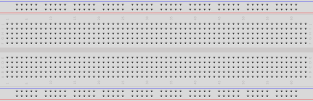
\includegraphics{bread_board.png}
		\caption[Bread board $n$.][6pt]{The preferred type of bread board. There are plenty of connections points and rails for dual supply voltage.}
		\label{fig:textfig}
	\end{figure}
	
	A basic supply of passive components will be needed for the projects and you can afterwards reuse most of these in your own projects. There starter kits that you can buy for around \$15. These kits can easily be found at the same places where you buy your ESP32 development kit. Search for "Arduino starter kit" or "bread board starter kit".
	
\end{document} 